\documentclass[12pt]{article}
 \usepackage[margin=1in]{geometry} 
\usepackage{amsmath,amsthm,amssymb,amsfonts}
\usepackage{graphicx}

 
\newcommand{\N}{\mathbb{N}}
\newcommand{\Z}{\mathbb{Z}}
 
\newenvironment{problem}[2]{\begin{trivlist}
\item[\hskip \labelsep {\bfseries #1}\hskip \labelsep {\bfseries #2.}]}{\end{trivlist}}

 
\begin{document}
  
\title{Computational Physics Project 1: Pendulum}
\author{Ben Zager, Remy Wang}
\maketitle
 
\begin{problem}{1}
	Phase space of unmodified nonlinear pendulum

\begin{figure}[h!]
  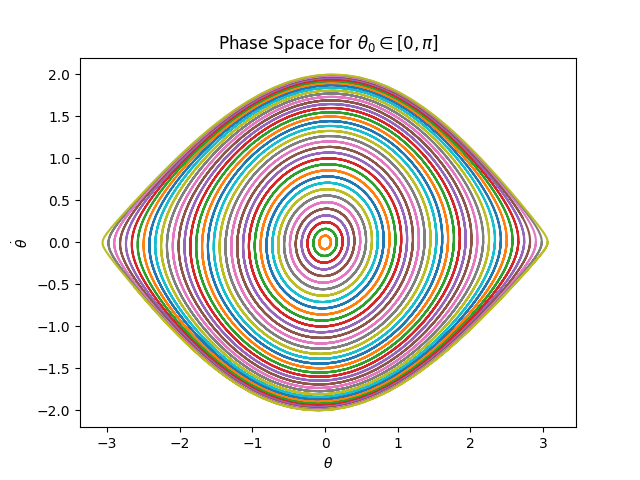
\includegraphics[scale=0.7]{figures/phaseSpace.png}
  \caption{Plots of trajectory $(\theta,\dot{\theta})$, for many values of $\theta_{0} \in [0,\pi]$}
  \label{fig:phase1}
\end{figure}

\begin{figure}[h!]
	\centering
	\begin{minipage}[b]{0.4\textwidth}
		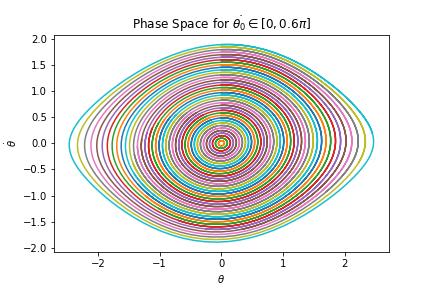
\includegraphics[scale=0.6]{figures/phaseSpaceDot.png}
		\label{phaseDot}
	\end{minipage}
	\hfill
	\begin{minipage}[b]{0.4\textwidth}
		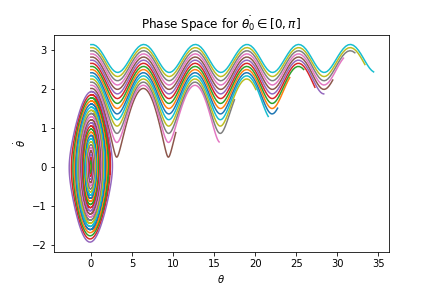
\includegraphics[scale=0.6]{figures/phaseSpaceDot2.png}
		\label{phaseDot2}
	\end{minipage}
	\caption{Trajectory for various $\dot{\theta}$}
\end{figure}
\end{problem}
 
\begin{problem}{2}
	Phase space of linear pendulum
\begin{figure}[h!]
  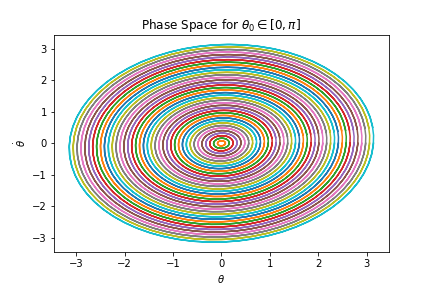
\includegraphics[scale=0.7]{figures/phaseSpaceLinear.png}
  \caption{Plots of trajectory $(\theta,\dot{\theta})$, for many values of $\theta_{0} \in [0,\pi]$}
  \label{fig:phase1}
\end{figure}
\end{problem}

\begin{problem}{3}
	Pendulum with driving force
\end{problem}

\begin{problem}{4}

\end{problem}

\begin{problem}{5}

\end{problem}

\begin{problem}{6}

\end{problem}

\begin{problem}{7}

\end{problem}


\end{document}